\documentclass{article}
\usepackage[utf8]{inputenc}
\usepackage{amsmath}
\usepackage{amssymb}
\usepackage{amsthm}

\usepackage{amsmath}
\usepackage{amssymb}
\usepackage{amsthm}
\usepackage{amscd}
\usepackage{amsfonts}
\usepackage{mathtools}

\usepackage[
backend=biber,
style=alphabetic,
sorting=ynt
]{biblatex}


\newtheorem{proposition}{Proposition}
\newtheorem{remark}{Remark}


\newcommand{\RR}[0]{\mathbb{R}}
\newcommand{\EE}[0]{\mathbb{E}}
\newcommand{\bx}[0]{{\bf x}}
\newcommand{\bv}[0]{{\bf v}}
\newcommand{\balpha}[0]{{ \bf\alpha}}
\newcommand{\HamiltonJacobiPDE}[2]{
%#1: Value function, #2: independent running cost
#1_t (x,t) + H(x,D_x #1(x,t)) = #2
}
\newcommand{\HamiltonJacobiTerminalCondition}[2]{
%#1: Value function, #2: Terminal payoff
#1(x,T) = #2(x)
}


\newcommand{\DensityTransportPDE}[2]{
    % #1: Value function, #2: Density
    #2_t(x,t) + \Delta(H_p(x, D_x #1 (x,t)) #2(x,t)) = 0
}

\newcommand{\DensityTransportInitialCondition}[1]{
    % #1: Density
    #1(x,t_0) = #1_0(x)
}


\newcommand{\ReducedMfgStateEvolution}[2]{
\begin{equation}\label{reduced_mfg:state_evolution}
\begin{cases}
    \dot{ #1}_t = {#2}_t,\quad t\in (t_0,T],\\
    {#1}_{t_0} = #1_0.
\end{cases}
\end{equation}
}

\newcommand{\ReducedMfgPayoffFunctional}[5]{
\begin{equation}\label{reduced_mfg:payoff_functional}
J({\bf #2},#1; t_0) = \int_{t_0}^T \left(#3({\bf #2}_s,{\bf #1}_s) + #5 \right) ds + #4({\bf #1}_T),
\end{equation}}

\newcommand{\ReducedMfgHamiltonian}[4]{
\begin{equation}\label{reduced_mfg:HJ}
H(#1,#2) \coloneqq \sup_{#3} ( #2 \cdot #3 + #4(#3,#1)).
\end{equation}
}


\newcommand{\ReducedMfgStateHamiltonJacobiTerminalValueProblem}[3]{
\begin{equation}\label{reduced_mfg:state_evolution_hamiltonian}
\begin{cases}
    \HamiltonJacobiPDE{#1}{#2}, \\
    \HamiltonJacobiTerminalCondition{#1}{#3}.
\end{cases}
\end{equation}}

\newcommand{\ReducedMfgFeedbackStateEvolution}[3]{
\begin{equation}\label{reduced_mfg:feedback_state_evolution}
\begin{cases}
    {\dot {\bf #1}}_#2 = H_p({\bf #1}, D_x #3({\bf #1},#2)),\\
    {\bf #1}_{t_0} = #1.
\end{cases}
\end{equation}}


\newcommand{\ReducedMfgDensityTransportInitialValueProblem}[2]{
\begin{equation}\label{reduced_mfg:density_transport_pde}
\begin{cases}
    \DensityTransportPDE{#1}{#2},\\
    \DensityTransportInitialCondition{#2}
\end{cases}
\end{equation}}

\newcommand{\ReducedMfgMeanFieldGameSystem}[4]{
\begin{equation}\label{reduced_mfg:mean_field_game_pde}
\begin{cases}
    \HamiltonJacobiPDE{#1}{#4},\\
    \DensityTransportPDE{#1}{#2},\\
\end{cases}
\end{equation}}

\newcommand{\ReducedMfgMeanFieldGameBoundaryConditions}[4]{
\begin{equation}\label{reduced_mfg:mean_field_game_boundary}
\begin{cases}
    \HamiltonJacobiTerminalCondition{#1}{#3},\\
    \DensityTransportInitialCondition{#2}.
\end{cases}
\end{equation}}



\addbibresource{sample.bib}
\addbibresource{sample.bib}

\title{A Mean Field Game Model For Educational Choices}
\author{Felipe Antunes}
\date{\today}

%"The great wish of some is to avenge themselves on some particular
%enemy, the great wish of others is to save their own pocket.  Slow
%in assembling, they devote a very small fraction of the time to the
%consideration of any public object, most of it to the prosecution of
%their own objects.  Meanwhile each fancies that no harm will come of
%his neglect, that it is the business of someone else to look after
%this or that for him; and so, by the same notion being entertained
%by all separately, the common cause imperceptibly decays".
% Thucydides - "The history of the Peloponnesian War"


\begin{document}

\maketitle


\section{Introduction}
Mean field games is a branch of game theory, which is a set of concepts, mathematical tools, theorems, simulations methods and algorithms intended to model situations where agents make decisions strategically. Mean field game theory focus specifically a game with an infinite number of identical (symmetric) players. The infinite number of players are represented by their probability distribution over the state (or action) space.

Analysis of MFG focus on the interaction between a representative player sampled from the distribution, and the distribution itself. In essence, the representative player formulates his best response to the crowd. However, as every player is equal, the best response of the representative player determines the evolution of the crowd.


Applications focus mostly on Nash equilibria or social optimum, respectively mean field game and mean field control.
Mean field games concern the "competitive" setting, where each player decides his actions by means of solving  his own optimization problem. Mean field control, on the other hand, describe the "cooperative" setting, where the player's actions are derived from an optimization problem on the player's distribution as a whole. 

As an illustrative example, consider crowd motion: a crowd in a music festival could be modelled as a mean field game, with each individual attempting to optimize his position considering the loudness and the crowd's density. However, a military parade could be modelled as a mean field control, with each individual given orders to follow by a commander who wants to optimize the troop's distribution. 

In both cases, the optimality conditions give rise to coupled equations with a forward-backward structure: the forward equation describe the evolution of the distribution of players, while the backward equation describes the optimization problem for the representative player. The problem can be formulated in an analytical approach or in a probabilistic approach. 
In the analytical formulation, we have a system composed of a Fokker-Plank PDE with initial condition and a Hamilton-Jacobi-Bellman PDE with terminal condition \cite{lasry2007mean}.
As for the probabilistic formulation, we have a system of Forward-Backward SDE with McKean-Vlasov interactions \cite{carmona2013mean}. 

\if{
Some fields of application for MFG are 
\begin{itemize}
    \item economics: financial engineering [citations] and macroeconomic models [citations],
    \item population dynamics [citations], crowd motion [] and epidemiology [citations]
    \item engineering: energy production and management [citations], security and communication [citations], autonomous vehicles [citations].
\end{itemize}
}\fi


\subsection{An example from economics}
%%%%%%WIP%%%%%

We will consider an example from economics in order to illustrate the mean field games methodology.
The example will be analyzed in a informal manner, aiming to introduce the general idea
of MFGs.
This model was chosen as an example for two reasons.
First, the mean field interactions arise naturally from the underlying economic theory, which makes the example a fitting introduction.
Second, the model is similar in nature to the educational model that we shall propose in Section~\ref{model_proposal}.
The example will be formulated in the deterministic setting, where the Nash equilibrium can be described using Pontryagin's Maximum Principle 
as the solution to a system of forward-backwards ODEs.

Consider an idealized economy composed of $N$ agents, with an optimization interval from time $t = 0$ to $t = T$.
Each agent has an amount of capital $k_0^i$ for $i \in \{1,\ldots,N\}$ at time $0$,
and they're able to control their consumption $c_t^i \in \RR$ over time.
The capital dynamics over time $d k_t^i$ is governed by
two factors besides the consumption:
a fixed depreciation rate $\delta$ and an endogenous interest rate $r_t$.
It is given by the ODE
\begin{equation}
    \dot k_t^i =  \left( \left[r_t - \delta \right] k_t^i - c_t^i \right)\, dt.
\end{equation}

Let us assume that the aggregate production $Y_t$ in the economy is given by a function $F$ of the aggregate capital of the economy $\hat k_t$, that is
\begin{equation}
    Y_t = F(\bar k_t),\quad \text{where } \bar k_t = \frac{1}{N} \sum_{i = 1}^N k_t^i.
\end{equation}
In economic equilibrium, the interest rate $r_t$ will be determined by the marginal effect of capital $\partial_K Y$ in the aggregate production,
which itself is a function of the aggregate capital in the economy $\bar k_t$.
This will be the source of the mean field interactions of our model.

The preference for consumption of the agents is given by an utility function $u(c_t^i)$, 
and their preference for capital at the end of their lifetime is given by a terminal utility $\psi(k_T^i)$.
Therefore, agents want to choose their measurable consumption function $c : [0,T] \mapsto \mathbb{R}$ to optimize the following functional $J(k, c)$:
\begin{equation}
    J(k, c) = \int_0^T u(c_s) ds + \psi(k_T),
\end{equation}
where $k$ is the starting capital, and $k_T$ is the capital at time $T$ when following control $c(\cdot)$.
Therefore, the optimization problem faced by agent $i$ is
\begin{equation}\label{economic_example:N_player_game}
    \begin{cases}
        \max_{c^i } \int_0^T u(c^i_s) ds + \psi(k^i_T),\\
        \text{subject to}\\
        d k_t^i = \left[\left( \partial_K F(\bar k_t) - \delta \right) k_t^i - c_t^i\right]\, dt.
    \end{cases}
\end{equation}

In the mean field game framework, instead of directly solving the $N$-player model~\eqref{economic_example:N_player_game},
we solve a different but related problem. 
We modify the setting of the game from $N$ players distributed at time $t$ according 
to a discrete probability measure flow $\mu^N_t = \frac{1}{N} \sum_{i = 1}^N \delta_{k^i_t}$
to infinite players distributed according to a (possibly atomless) probability measure flow $\mu_t$.
This new setting is the mean field game approximation of the original game.

Recall that a Nash equilibrium is a combination of the players' states in which 
no player can improve its outcome by changing its actions.
If we consider a time evolution for the players' population given by $\mu_t$,
each player can formulate its best response
(that is, its optimal consumption $c^*$) when the population evolves according to
$\mu_t$.
However, the best response of each player \textit{induces}
a new population evolution described by another probability measure flow $\nu_t$.
If there exists a probability measure flow $\mu_t^*$ such that the best response
of each player induces itself, this means that under $\mu_t^*$,
\textit{no player can improve its outcome by changing its actions.}
Therefore, if a probability measure flow $\mu_t^*$ exists, we interpret it as
the Nash equilibrium of the MFG, coinciding with the classical definition.

We're now in position to analyze the model. Analysis of mean field games models have the following pattern:
\begin{enumerate}
    \item Find the optimal control for a representative player, given a flow of probability measures $\mu_t$,
    \item As every player is equal, their optimal trajectories induce a flow $O(\mu_t)$,
    \item A Nash equilibrium for the MFG is a probability flow $\mu_t^*$ such that $\mu_t^* = O(\mu_t^*)$.
\end{enumerate}
%By definition, a Nash equilibrium is a state of the game where no player can improve his outcome by unilaterally changing his strategy.
%The measure flow $\mu_t^*$ induces its own time evolution when every player behaves optimally.
%This means they can't improve their outcomes any more,
%which means that the mean field definition of Nash equilibrium is compatible with the classical definition.
 
Let us set $u(c) = \log(c)$ and $\psi(k) = - \frac{1}{2} k^2$.
Moreover, denote $\bar k_t = \int k d \mu_t(k)$ and set $F(K) = \frac{C}{2} K^2$, that is, there are increasing returns over aggregated capital.
In this setting, the interest rate is given by $r_t = C {\bar k_t} $.
Assuming that an initial capital distribution $\mu_0$ is given,
the representative agent faces the following optimization problem:
\begin{equation}\label{economic_example:representative_agent}
    \begin{cases}
        \max_{c} \int_0^T \log(c_s) ds -\frac{1}{2}{(k_T)}^2,\\
        \text{subject to}\\
        d {\bar k}_t = \left(\left[ C {\bar k_t} - \delta \right] k_t - c_t \right) dt, \quad k_0 \sim \mu_0,
    \end{cases}
\end{equation}

Assuming that ${\bar k_t}$ is given, we can apply Pontryagin's Maximum Principle~\cite{bressan2007introduction}
to conclude that, if an optimal control $c^*$ and a corresponding optimal trajectory $k^*$ exist,
then there is a costate variable $p$ defined implicitly as the solution of the backwards ordinary differential equation
\begin{equation}\label{economic_example:costate_ode}
    d p_t = -  \left[C{{\bar k}_t} - \delta \right] p_t\, dt, \quad p_T =  - k^*_T,
\end{equation}
that satisfy the maximality condition
\begin{equation}\label{economic_example:maximality_condition}
    p_t\left( \left[C {\bar k_t} - \delta \right]k^*_t - c^*_t \right) + \log(c^*_t) = 
    \max_{c \in \mathbb{R}^+} \left\{ p_t\left( \left[C {\bar k_t} - \delta \right]k^*_t - c \right) + \log(c) \right\}.
\end{equation}

We can find candidates for optimal controls and trajectories by calculating
\begin{equation*}
    c^* = \arg\max_{c \in \mathbb{R}^+}  \left\{ p_t\left( \left[C {\hat k_t} - \delta \right]k^*_t - c \right) + \log(c) \right\} = \frac{1}{p_t},
\end{equation*}
and solving the forward-backward system of ordinary differential equations
\begin{equation}\label{economic_example:ode_formulation}
    \begin{cases}
         d k_t = \left(\left[ C {\hat k_t} - \delta \right] k_t - \frac{1}{p_t} \right)\, dt,\\
         d p_t = - \left( \left[C{\hat k_t} - \delta \right] p_t \right) \, dt, \\
         k_0 \sim \mu_0,\, p_T =  - k_T.         
    \end{cases}
\end{equation}
    Note that $k_t$ is actually a random variable dependent on its initial distribution $\mu_0$.
    The system of ODEs implicitly describes the probability measure flow $\mu_t = \mathcal{L}(k_t)$,
    and the dynamics of this forward-backward system depend on $\mathcal{L}(k_t)$ through $\bar k_t$.
    In the stochastic case, the dependence on the law is the distinguishing feature of McKean-Vlasov SDEs.

    Pontryagin's Maximum Principle give us \textit{necessary} conditions for optimal controls and trajectories, but not \textit{sufficient} conditions.
    In order to guarantee optimality, one method is to analyze the value function $V$ defined as
\begin{equation}\label{economic_example:value_function_definition}
    V(k,t) = \sup_{c,\, k_t = k} \int_t^T \log(c(s)) ds -\frac{1}{2}{(k_T)}^2.
\end{equation}
Intuitively, the value function evaluates for a given time $t$ and capital $k$ the optimal payoff from that point forward.
As shown in section~\ref{theo_review:soc}, the value function is the viscosity solution for the Hamilton-Jacobi-Bellman equation
\begin{equation}\label{economic_example:hjb_equation_reduced}
    \begin{split}
        &\partial_t V + H(\partial_k V, k,t) = 0,\quad V(k,T) = -\frac{1}{2}{(k)}^2,\\
        &\text{where }
        H(p,k,t) = \sup_{c \in \mathbb{R}^+} \left\{ p\left[ \left(C {\hat k_t - \delta}\right)k - c \right] + \log(c) \right\}.
    \end{split}
\end{equation}
This equation encodes the system of ODEs in~\ref{economic_example:ode_formulation} through the Hamiltonian function by the relations
\begin{equation*}
    d k_t = \partial_p H\, dt ,\quad d p_t = -\partial_k H \, dt.
\end{equation*}
Moreover, as shown in~\ref{theo_review:wass},
when the agents' capital evolve according to $d k = \partial_p H\, dt$,
the probability density function $\rho(\cdot, t)$ for the agents probability measure $\mu_t$ at time $t$
is the weak solution for the Kolmogorov-Fokker-Planck equation with initial condition $\rho_0$ given by the pdf of $\mu_0$
\begin{equation}\label{economic_example:fkp_equation_reduced}
\begin{split}
    &\partial_t \rho - \partial_k \left( \partial_p H \rho \right) = 0, \quad\rho(k,0) = \rho_0.
\end{split}
\end{equation}
In the Nash Equilibrium, the capital per capita at time $t$ is a function of $\rho$ given by $\bar k_t(\rho) = \int_{\RR} k \rho(k,t) dk$.
Substituting 
\begin{equation*}
    H(p,k,t) = \left(C {\bar k_t(\rho) - \delta}\right)k p  - 1  - \log(p),
\end{equation*}
on~\ref{economic_example:hjb_equation_reduced} and~\ref{economic_example:fkp_equation_reduced}, we have the full PDE system
\begin{equation}
    \begin{cases}
        \partial_t V +  \left(C {\bar k_t(\rho) - \delta}\right)k\partial_k V - 1  - \log(\partial_k V) = 0,  \quad V(k,T) = -\frac{1}{2}{(k)}^2,\\
        \partial_t \rho - \partial_k \left( \left[ \left(C {\bar k_t}(\rho) - \delta\right) k - {(\partial_k V)}^{-1} \right]\rho \right) = 0, \quad \rho(k,0) = \rho_0.
    \end{cases}
\end{equation}
\color{black}




\section{Theoretical Review - Mean Field Games Theory}


Mean field games are a framework for approximating Nash equilibria of certain kinds of games with a large number of players.
There are two equivalent ways of formulating a mean field game - through a system of coupled partial differential equations, or through a system of forward-backward stochastic differential equations.

In this section, we will explore the theory of mean field games.
We will begin by reviewing important prerequisites - namely stochastic optimal control in . 
Then, we shall review both the PDE system point of view and the FBSDE point of view. 
Equiped with an understanding of both point of views, we will analyze the limit of N-player games and its relationship to MFG.
Following the theoretical subsections, we will explore numerical solutions for MFG and applications.
We shall end the section by analyzing a model for human capital development.
We refer the reader to Appendix \ref{appendix-game-theory} for a review of game theory concepts, and to Appendix \ref{appendix-mathematical-background} for a review of necessary mathematical background.


\if{
\subsection{Three roads for Mean Field Games Theory}

Conceptually, there are three approaches to mean field games theory - from physics, from game theory and from economic theory.

\subsubsection{First road: from physics to mean field games}

% To do
% Add an physical example - i.e. gravity vs termal pressure model
In particle physics, situations with large number of particles are handled using mean field theory. Instead of modelling all the inter-particle interactions, one introduces a "mean field" which serve as mediator for the interactions. Each particle both contributes to and is influenced by the mean field.

In order to use this approximation, the inter-particle interactions must be sufficiently weak or regular.

Mean field game theory adapts this methodology to situations in which agents interact in strategic situations. The challenge is to take into account not only the ability of agents to make decisions, but also the interaction between strategies: each player's strategy tries to take into account the other player's strategy.
\textbf{This changes the nature of the mean field: it is not an statistic on the domain of particle states anymore, but rather a statistic on the domain of strategies and information.}

Although the term "mean-field" is borrowed from Physics, mean field game theory does not restrain itself to applying physical models to economy. Instead, as a branch of game theory, mean field games models aim to \textit{explain} rational behaviour through the structure of the agent's interactions and payoffs. \cite{cousin2010paris}

\subsubsection{Second Road: From Game Theory to Mean Field Games}

In game theory, $N$-player games quickly become intractable as $N$ gets large. Mean Field Games provide a way to approximate the limiting case as $N \to \infty$ for a class of $N$-player game which respect a form of anonymity: direct interactions between players are comparatively small, and players can be interchanged without changing the interaction. This is the case when interactions are mediated through some average of the player's state, for instance.
The mean field approach consists in approximating the $N$ players by a continuum of players distributed through the state space. Each agent formulates his optimal response given the distribution of players, and conversely this optimal response implies an evolution through time for the player's distribution.
\textit{In layman's terms, each player formulates his strategy against the crowd, and the crowd evolves according to each player's strategy.}

\subsubsection{Third Road: From Economics to Mean Field Games}
% To Do
% Add toy model with general equilibrium, reference it here
In economic models following the Theory of General Economic Equilibrium, interactions are mediated by prices. Direct interactions of agents are excluded from these economic models. However, systemic economic effects such as externalities, public goods, etc give rise to interactions which are not mediated by price. Both price formation and systemic effects can be modelled by a mean field type model. This way, MFG theory lends itself as a tool of economic analysis.
}\fi

\subsection{Stochastic Optimal Control}\label{theo_review:soc}

This section is a compendium of stochastic control.
We follow~\cite{pham2009continuous} and present briefly the necessary results
for a full understanding of MFG theory.

Consider a system governed by the controlled
stochastic differential equation (SDE) in $\RR^n$:
\begin{equation}\label{soc:controlled_sde}
    d X_s = b(X_s, \alpha_s)ds + \sigma(X_s, \alpha_s) d W_s
\end{equation}
where $W$ is a $d$-dimensional Brownian motion on a filtered probability space
$(\Omega, \mathcal{F}, \mathbb{F} = {(\mathbb{F}_t)}_{t \geq 0}, \mathbb{P} )$ satisfying the
usual conditions.
The coefficients $b(t,x,a)$ and $\sigma(t,x,a)$ are depend on $t$, except
in the case of infinite horizon problems.
The control $\alpha = (\alpha_s)$ is a progressively measurable process w.r.t.
$\mathbb{F}$, valued in $A \subset \RR^m$.

The functions $b: \mathbb{R}^n \times A \mapsto \mathbb{R}^n$ and 
$\sigma: \mathbb{R}^n \times A \mapsto \RR^{n\times d}$ are uniformly
Lipschitz over $A$: $\exists K \geq 0, \forall x,y, \in \RR^n, \forall a \in A$,
\begin{equation}\label{soc:diffusion_uniformly_lipschitz}
    | b(x,a) - b(y,a) | + | \sigma(x,a) - \sigma(y,a) | \geq K | x - y |.   
\end{equation}

Fix a time $0 < T < \infty$, and let $\mathcal{A}$ be the set of control processes
$\alpha$ such that
\begin{equation}\label{soc:diffusion_quadratic_bound}
    \mathbb{E}\left[ \int^T_0 |b( 0,\alpha_t )|^2 + |\sigma( 0, \alpha_t )|^2 dt \right] < \infty.
\end{equation}

Conditions~\eqref{soc:diffusion_uniformly_lipschitz} 
and~\eqref{soc:diffusion_quadratic_bound} ensure the existence and uniqueness
of a strong solution to the SDE~\eqref{soc:controlled_sde}
for every control $\alpha \in \mathcal{A}$ and for every initial condition
$(t,x) \in [0,T] \times \RR^n$, and we denote by $\{ X_s^{t,x}, t \leq s \leq T \}$
this solution with a.s.\ continuous paths. Moreover, under these conditions,
it follows that
    \begin{gather}
        \mathbb{E} \left[ \sup\limits_{t\leq s \leq T} \right] < \infty,\\
        \lim_{h \to 0^+} \mathbb{E} \left[ \sup\limits_{s\in [t,t+h]} | X_s^{t,x} - x |^2 \right] = 0.
    \end{gather}

We now turn to the definitions of the objective function and the value function.
Let $ f: [0,T] \times \RR^n \times A \mapsto \RR $ and $ g: \RR^n \mapsto \RR $
be two measurable functions. Assume that is either $g$ lower-bounded or 
satisfies a quadratic growth condition 
$| g(x) | \leq C(1 + |x|^2),\ \forall x \in \RR^n$, for some constant $C$
independent of $x$.

For $(t,x) \in [0,T] \times \RR^n$, let $\mathcal{A}(t,x) \subset \mathcal{A}$
be such that, $\forall \alpha \in \mathcal{A}(t,x)$
\begin{equation}
    \mathbb{E}\left[ \int_t^T | f(s, X_s^{t,x}, \alpha_s) | ds \right] < \infty,
\end{equation}
and assume $\mathcal{A}(t,x)$ is not empty for all
$(t,x) \in [0,T] \times \RR^n$.

We can now define the objective function $J$
\begin{equation}
    J(t, x, \alpha) = \mathbb{E}\left[ \int_t^T f(s, X_s^{t,x}, \alpha_s) ds + g(X^{t,x}_T) \right],
\end{equation}
for all $(t,x) \in [0,T] \times \RR^n$ and $\alpha \in \mathcal{A}(t,x)$.
We want to maximize over the controlled processes the objective function, so
we introduce the associated value function $v$:
\begin{equation}
    v(t,x) = \sup_{\alpha \in \mathcal{A}(t,x)} J(t,x,\alpha).
\end{equation}
Given an initial condition $(t,x) \in \left[ 0,T \right) \times \RR^n$, we say
that $\hat \alpha \in \mathcal{A}(t,x)$ is an optimal control if
$v(t,x) = J(t,x,\hat \alpha)$.
Moreover, a control process $\alpha$ in the form $\alpha_s = a(s,X_s^{t,x})$ for
a measurable function $a: [0,T] \times \RR^n \mapsto A$ is
called a Markovian control.

We are now in position to state a fundamental property of the value function $v$,
called the \textit{Dynamic Programming Principle}:

\begin{theorem}[Dynamic Programming Principle]
    Let $(t,x) \in [0,T] \times \RR^n$. The value function $v$ satisfies
\begin{gather} 
        v(t,x) = \sup_{\alpha \in \mathcal{A}(t,x)}
        \sup_{\theta \in \mathcal{T}_{t,T}}
        \mathbb{E}\left[ \int_t^\theta f(s, X_s^{t,x}, \alpha_s) ds + v(\theta, X^{t,x}_\theta) \right]\\
        =\sup_{\alpha \in \mathcal{A}(t,x)}
        \inf_{\theta \in \mathcal{T}_{t,T}}
        \mathbb{E}\left[ \int_t^\theta f(s, X_s^{t,x}, \alpha_s) ds + v(\theta, X^{t,x}_\theta) \right]
\end{gather}
    where $\mathcal{T}_{t, T}$ is the set of stopping times valued in $[t,T]$.
\end{theorem}

\begin{proof}
    Given an admissible control $\mathcal{A}(t,x)$, by pathwise uniqueness of the flow of the SDE for $X$ we have
    \begin{equation}
        X_s^{t,x} =  X_s^{\theta, X_\theta^{t,x}}, \, s \geq \theta
    \end{equation}
    for any stopping time $\theta \in [t,T]$. By the tower property of expectations, 
    we have
    \begin{align*}
        J(t,x,\alpha) &= \mathbb{E}\left[ \int_t^T f(s, X_s^{t,x}, \alpha_s) ds + G(X_T^{t,x})  \right] \\
        &= \mathbb{E}\left[ \mathbb{E} \left[ \int_t^T f(s, X_s^{t,x}, \alpha_s) ds + G(X_T^{t,x}) | \mathcal{F}_\theta \right] \right] \\
        &= \mathbb{E}\left[  \int_t^\theta f(s,X_s^{t,x}, \alpha_s) ds +  \mathbb{E} \left[ \int_\theta^T f(s, X_s^{t,x}, \alpha_s) ds + G(X_T^{t,x}) | \mathcal{F}_\theta \right] \right]\\ 
        &= \mathbb{E}\left[  \int_t^\theta f(s,X_s^{t,x}, \alpha_s) ds +  J(\theta, X_\theta^{t,x}, \alpha) \right].
    \end{align*}
    By the definition of the value function $v$, $J(t,x,\alpha) \leq v(t,x)$.
    Moreover, as $\theta$ is arbitrary in $\mathcal{T}_{t,T}$, we have
    \begin{align*}
        J(t,x,\alpha) &\leq \inf_{\theta \in \mathcal{T}_{t,T}} \mathbb{E}\left[ \int_t^\theta f(s, X_s^{t,x}, \alpha_s) ds  + v(\theta, X_\theta^{t,x})\right] \\
        & \leq \sup_{\alpha \in \mathcal{A}(t,x)} \inf_{\theta \in \mathcal{T}_{t,T}} \mathbb{E}\left[ \int_t^\theta f(s,X^{t,x}_s, \alpha_s) ds + v(\theta, X_\theta^{t,x}) \right]. 
    \end{align*}
    by taking the supremum over $\alpha$ in the left side, we conclude that
    \begin{equation}
        v(t,x)  \leq \sup_{\alpha \in \mathcal{A}(t,x)} \inf_{\theta \in \mathcal{T}_{t,T}} \mathbb{E}\left[ \int_t^\theta f(s,X^{t,x}_s, \alpha_s) ds + v(\theta, X_\theta^{t,x}) \right]. 
    \end{equation}
    Now, for the other side of the inequality: fix some arbitrary control
    $\alpha \in \mathcal{A}(t,x)$ and $\theta \in \mathcal{T}_{t,T}$.
    By definition of the value functions, for any $\epsilon > 0$ and 
    $\omega in \Omega$, there exists an $\epsilon$-optimal control
    $\alpha^{\epsilon, \omega} \in \mathcal{A}( \theta(\omega), X^{t,x}_{\theta(\omega)} (\omega)  )$
    such that
\begin{equation}\label{soc:dpp_proof_epsilon_optimal_control}
    v(\theta(\omega), X^{t,x}_{\theta(\omega)}(\omega)) - \epsilon \leq J(\theta(\omega), X^{t,x}_{\theta(\omega)}(\omega), \alpha^{\epsilon, \omega}).
\end{equation}    
    We can define the process
\begin{equation*}
    \hat\alpha_s(\omega) = 
    \begin{cases}
        \alpha_s(\omega), s \in [0,\theta(\omega)],\\
        \alpha_s^{\epsilon, \omega}(\omega), s \in [\theta(\omega), T].
    \end{cases}
\end{equation*}
As stated in~\cite{pham2009continuous}, it can be shown that $\hat \alpha$ is progressively measurable,
so it lies in $\mathcal{A}(t,x)$.
Again, by the tower property and by inequality~\eqref{soc:dpp_proof_epsilon_optimal_control}
\begin{align*}
    v(t,x) &\geq J(t,x, \hat \alpha) = \mathbb{E}\left[ \int_t^\theta f(s,X^{t,x}_s, \alpha_s) ds + J(\theta, X^{t,x}_\theta, \alpha^\epsilon) \right] \\
            &\geq \mathbb{E}\left[ \int_t^\theta f(s,X^{t,x}_s, \alpha_s) ds + v(\theta, X^{t,x}_\theta) \right] - \epsilon.
\end{align*}
As $\alpha, \theta$ were arbitrary, we conclude that
\begin{equation}
    v(t,x) \geq \sup_{\alpha \in \mathcal{A}(t,x)} \sup_{\theta \in \mathcal{T}_{t,T}} \mathbb{E} \left[ \int_t^\theta f(s, X_s^{t,x}, \alpha_s) ds + v(\theta, X^{t,x}_\theta) \right].
\end{equation}
Combining both inequalities concludes the proof.
\end{proof}

From the dynamic programming principle, we can derive the Hamilton-Jacobi-Bellman (HJB)
equation. The HJB equation is an infinitesimal version of the DPP, which describes
the local behaviour of the value function.

Consider the time $\theta = t + h$ and a constant control $\alpha_s = a$, for some
arbitrary $a \in A$. From the statement of the DPP, we have
\begin{equation}\label{soc:dpp_ineq}
    v(t,x) \geq \mathbb{E}\left[ \int_t^{t + h} f(s,X^{t,x}_s,a) ds + v(t+h, X^{t,x}_{t+h}) \right]
\end{equation}
By assuming smoothness of $v$, we can apply Ito's formula between $t$ and $t+ h$:
\begin{equation*}
    v(t+h, X^{t,x}_{t+h}) = v(t,x) + \int^{t+h}_t \left( \frac{\partial v}{\partial t} + \mathcal{L}^a v\right)(s, X^{t,x}_s) ds + \int_t^{t+h} \frac{\partial v}{\partial x} (s, X^{t,x}_s) dW_s,
\end{equation*}
where $\mathcal{L}^a$ is the operator associated with the
diffusion~\eqref{soc:controlled_sde}, defined by
\begin{equation}
    \mathcal{L}^a v = b(x,a) \partial_x v + \frac{1}{2}\text{tr} (\sigma(x,a) \sigma'(x,a) \partial_{xx}v).
\end{equation}
By substituting back into~\eqref{soc:dpp_ineq}, we have
\begin{equation*}
    0 \geq \mathbb{E}\left[ \int^{t+h}_t \left( \frac{\partial v}{\partial t} + \mathcal{L}^a v\right)(s, X^{t,x}_s) + f(s, X^{t,x}_s, a)  ds\right]
\end{equation*}
We can divide by $h$, apply the mean value theorem and take $h\to 0$ to arrive at
\begin{equation*}
    0 \geq \frac{\partial v}{\partial t} (t,x) + \mathcal{L}^a v(t,x) + f(t,x,a).
\end{equation*}
Since this holds for any $a \in A$, we have that
\begin{equation}\label{soc:hjb_inequality}
    - \frac{\partial v}{\partial t} (t,x) - \sup_{a \in A} \left[ \mathcal{L}^a v(t,x) + f(t,x,a) \right] \geq 0.
\end{equation}

On the other hand, suppose that $\alpha^*$ is an optimal control.
Then equality is achieved in the DPP:
\begin{equation}
    v(t,x) = \mathbb{E}\left[ \int^{t+h}_t f(s, X^*_s, \alpha^*_s) ds + v(t + h, X^*_{t+h}) \right],
\end{equation}
where $X^*$ is the evolution of the system starting from $x$ at $t$, with control $\alpha^*$.
By the same procedure as above, we arrive at
\begin{equation}
    - \frac{\partial v}{\partial t} (t,x) - \mathcal{L}^a v(t,x) - f(t,x,a) = 0.
\end{equation}
which, combined with~\eqref{soc:hjb_inequality} allows us to conclude that
\begin{equation}
    - \frac{\partial v}{\partial t} (t,x) - \sup_{a \in A} \left[ \mathcal{L}^a v(t,x) + f(t,x,a) \right] = 0
\end{equation}
for every $(t,x) \in [0,T) \times \RR^n $ where the supremum in $a$ is finite.

If we define the Hamiltonian function $H : [0,T] \times \RR^n \times \RR^n \times \mathcal{S}_n \mapsto \RR$
by
\begin{equation}
    H(t,x,p,M) = \sup_{a \in A} \left[ b(x,a)\cdot p + \frac{1}{2} \text{tr} (\sigma \sigma' (x,a) M) + f(t,x,a) \right],
\end{equation}
we can rewrite the PDE as
\begin{equation}\label{soc:hjb_equation}
    -\frac{ \partial v}{\partial t} (t,x) - H(t,x,\partial_x v(t,x), \partial_{xx} v(t,x)) = 0
\end{equation}
which is the Hamilton-Jacobi-Bellman equation.
The PDE has a terminal condition given by
\begin{equation}
    v(T,x) = g(x), \forall x \in \RR^n,
\end{equation}
which results from the definition of $v$ at the time horizon $T$.

In order to derive the Hamilton-Jacobi-Bellman equation, we assumed smoothness
of the value function. However, this does not necessarily hold, even in simple
cases. To deal with this difficulty, the notion of viscosity solutions was 
introduced, which allows a rigorous formulation for the HJB to be given under
the assumption of local boundedness. Moreover, viscosity solutions satisfy a 
comparison principle, from which we can derive uniqueness of solutions.
We shall state the definition and uniqueness result here, and
 refer to~\cite{pham2009continuous,bressan2007introduction,lopes1997introduccao} for a deeper exposition, 
 and to~\cite{crandall1992user} for a seminal reference to the topic.

 Let's consider the first order case, with a PDE of the form
 \begin{equation*}
    F(x,u, D u) = 0, x \in \Omega \subset \RR^n
 \end{equation*}
the theory of viscosity solutions show that the solutions $u^\epsilon(\cdot)$
to the equation
\begin{equation*}
    F(x, u^\epsilon, D u^\epsilon) = \epsilon \Delta u^\epsilon
\end{equation*}
converge to a unique limit $u(\cdot)$ as $\epsilon \to 0+$.
This limit is the viscosity solution to the PDE.
Moreover, the viscosity solution $u$ can be uniquely characterized by inequalities
in the superdifferential set $D^+ u(x)$ and the subdifferential set $D^- u(x)$
as follows:
\begin{itemize}
    \item A function $u \in C(\Omega)$ is a viscosity subsolution if
\begin{equation*}
    F(x, u(x), p) \leq 0, \text{ for every } x \in \Omega, p \in D^+ u(x).
\end{equation*}
    \item A function $u \in C(\Omega)$ is a viscosity supersolution if
\begin{equation*}
    F(x, u(x), p) \geq 0, \text{ for every } x \in \Omega, p \in D^- u(x).
\end{equation*}
    \item A function $u \in C(\Omega)$ is a viscosity solution if it is both
    a viscosity supersolution and a viscosity subsolution.
\end{itemize}
We can characterize the superdifferential (respectively the subdifferential) in
terms of test functions $\phi \in C^1(\Omega)$:
\begin{lemma}
    Let $u \in C(\Omega)$ and $x_0 \in \Omega$. Then $p_0  \in D^+ u(x_0)$ if and 
    only if there exists $\phi \in C^1(\Omega)$ such that:
\begin{enumerate}
    \item $u - \phi$ has a local maximum in $x_0$;
    \item $(u - \phi)(x_0) = 0$;
    \item $D \phi(x_0) = p_0$;
\end{enumerate}
\end{lemma}
For $p_0 \in D^- u(x_0)$, instead of a local maximum we have a local minimum.
This allows us to give an equivalent definition of viscosity solutions in terms 
of test functions. In fact, for second-order PDEs
of the form
\begin{equation}
    F(x, u, D u, D^2 u) = 0,
\end{equation}
where $F$ is assumed to satisfy the ellipticity condition
\begin{equation}
    M \leq \hat M \rightarrow F(x,r,p,M) \geq F(x,r,p,\hat M),
\end{equation}
for all $x \in \Omega, r \in \RR, p \in \RR^n, M,\hat M \in \mathcal{S}_n$,
this definition can be extended by considering test functions in $C^2(\Omega)$:
\begin{definition}[Second Order Viscosity Solutions]
    \begin{itemize}
        \item An upper-semicontinuous function $u : \Omega \mapsto \RR$ is a viscosity subsolution if
    \begin{equation*}
        F(x_0, u(x_0), D \phi(x_0), D^2 \phi(x_0)) \leq 0,
    \end{equation*}
    for all $x_0 \in \Omega$ and for all $\phi \in C^2(\Omega)$ such that $x_0$ is a maximum point of $u - \phi$.
        \item A lower-semicontinuous function $u : \Omega \mapsto \RR$ is a viscosity supersolution if
    \begin{equation*}
        F(x_0, u(x_0), D\phi(x_0), D^2 \phi(x_0)) \geq 0,
    \end{equation*}
    for all $x_0 \in \Omega$ and for all $\phi \in C^2(\Omega)$ such that $x_0$ is a minimum point of $u - \phi$.
        \item A function $u : \Omega \mapsto \RR$ is a viscosity solution if it is both
        a viscosity supersolution and a viscosity subsolution.
    \end{itemize}
\end{definition}

\subsection{Wasserstein Spaces}\label{theo_review:wass}
This section is a compendium of the topology and differential structure of
Wasserstein spaces. We follow~\cite{cardaliaguet2010notes,ambrosio2005gradient,ambrosio2021lectures}.
Our goal is to characterize absolute continuous measure flows as solutions to the continuity equation,
and to define the derivative of function in Wasserstein space with respect to the measure.

Let $\Omega \subset \RR^n$, $\mathcal{P}(\Omega)$ be the set of Borel
probability measures on $X$, and $\mathcal{P}_2(\Omega) \subset \mathcal{P}(\Omega)$
be the set of probability measures $m$ such that $\int_\Omega |x|^2 dm(x) < + \infty$.

We can define a metric over $\mathcal{P}_2(\Omega)$ called the 
\textit{Wasserstein distance} by
\begin{equation}\label{prob_measures:wasserstein_distance}
    d_2(\mu, \nu) = \inf_{\gamma \in \Pi(\mu,\nu)} \left[ \int_\Omega |x - y|^2 d\gamma(x,y) \right]^{\frac{1}{2}}
\end{equation}
where $\Pi(\mu,\nu)$ is the \textit{coupling} between $\mu$  and $\nu$,
that is, the set of Borel probability measures on $\Omega \times \Omega$
such that $\gamma(A \times \Omega) = \mu(A)$ and $\gamma(\Omega \times A) = \nu(A)$
for any Borel set $A \subset \Omega$.

The Wassertestein distance is a special case of Monge-Kantorovich distances
\begin{equation*}
    d_p(\mu, \nu) = \inf_{\gamma \in \Pi(\mu, \nu)} \left[ \int_{\Omega^2} d^p(x,y) d\gamma(x,y)  \right]^{\frac{1}{p}}.
\end{equation*}
One important property of Monge-Kantorovich distances is the existence of at least
one optimal measure, that is, one $\hat  \gamma \in \Pi(\mu,\nu)$ such that
$d_p(m,m') = \left[ \int_{\Omega^2} d^p(x,y) d {\hat \gamma}(x,y) \right]^{\frac{1}{p}}$.
The measure $\hat \gamma$ is called optimal transport plan.

In the case of the Wasserstein distance, an stronger property is satisfied when 
$\mu$ is absolutely continuous: the optimal transport plan can be realized as
an \textit{optimal transport map}~\cite{cardaliaguet2010notes}.
\begin{theorem}[Existence of an optimal transport map]
    If $\mu \in \mathcal{P}_2(\Omega)$ is absolutely continuous, then,
    for any $\nu \in \mathcal{P}_2(\Omega)$, there exists a convex map 
    $\Phi: \Omega \mapsto \RR $ such that the measure
    $ (\text{id}, D\Phi)\sharp \mu $ is optimal for $d_2(\mu, \nu)$, and $\nu = D \Phi \sharp \mu$.

    Conversely, if the convex map $\Phi : \Omega \mapsto \RR$ satisfies $\nu = D \Phi \sharp \mu$,
    then the measure $(\text{id}, D\Phi)\sharp \mu$ is optimal for $d_ 2(\mu,\nu)$.
\end{theorem}
Here the symbol $\sharp$ denotes the push-forward of the measure with respect to the map,
that is, for $\psi : \Omega \mapsto \Omega$, $\psi \sharp \mu(A) = \mu(\psi^{-1}(A))$

Definition~\eqref{wass:absolutely_continuous_curves} 
and Theorems~(\ref{wass:metric_derivative},~\ref{wass:abs_continuity_and_continuity_eq}) are found in~\cite{ambrosio2005gradient}. 

\begin{definition}[Absolutely Continuous Curves in Wasserstein space]\label{wass:absolutely_continuous_curves}
    Let $v : (a,b) \mapsto \mathcal{P}_2(\Omega)$ be a curve.
    We say that $v$ is absolutely continuous if there exists
    $m \in L^1(a,b)$ such that
    \begin{equation}\label{wass:absolute_continuity}
        d(v(s), v(t)) \leq \int_s^t m(r) dr, \forall a < s \leq t < b.
    \end{equation}
\end{definition}

Among all choices of $m$ in~\eqref{wass:absolute_continuity}, there is a minimal
one, which describes the \textit{metric derivative} of the curve
\begin{theorem}[Metric derivative]\label{wass:metric_derivative}
    For any absolute continuous curve $v$ over $\mathcal{P}_2$, the limit
    \begin{equation}
        |v'|(t) \coloneqq \lim_{s \to t} \frac{d(v(s), v(t))}{|s - t|}
    \end{equation}
    exists for $\mathcal{L}$-a.e. $t \in (a,b)$. Moreover, the function
    $ t \mapsto |v'|(t) $ belongs to $L^1(a,b)$, is an admissible integrand for
    the right hand side of~\eqref{wass:absolute_continuity}, and it satisfies
    \begin{equation}
        |v'|(t) \leq m(t) \text{ for }\mathcal{L}\text{-a.e. } t \in (a,b),
    \end{equation}
    for each function $m$ satisfying~\eqref{wass:absolute_continuity}.
\end{theorem}

The next Theorem relates solutions to the continuity equation
\[\partial_t \mu_t + \nabla \cdot (v_t \mu_t) = 0,\]
where $\nabla \cdot (f) = \sum_{i = 1}^n \partial_{x_i} f$,
and absolute continuous curves over Wasserstein space. 

\begin{theorem}[Absolutely continuous curves and the continuity equation]\label{wass:abs_continuity_and_continuity_eq}
    Let $\mu_t : (a,b) \mapsto \mathcal{P}_2(\Omega)$ be an absolutely continuous
    curve and let $|\mu'| \in L^1(a,b)$ be its metric derivative.
    Then there exists a Borel vector field $v : (x,t) \mapsto v_t(x)$ such that
    \begin{equation}
        v_t \in L^2(\mu_t, \Omega), ||v_t||_{L^2(\mu_t, \Omega)} \leq |\mu'|(t)\text{ for a.e. } t \in (a,b)
    \end{equation}
    and $\mu_t$ is a weak solution to the continuity equation
    \begin{equation}
        \partial_t \mu_t + \nabla \cdot (v_t \mu_t) = 0.
    \end{equation}
    Conversely, if a a curve which is continuous w.r.t.~the narrow topology
    $\mu_t : (a,b) \mapsto \mathcal{P}_2(\Omega)$
    satisfies the continuity equation for some Borel velocity field $v_t$ with
    $||v_t||_{L^1(\mu_t, \Omega)} \in L^1(a,b)$ then $\mu_t$ is absolutely continuous
    and $ |\mu'|(t) \leq  ||v_t||_{L^1(\mu_t, \Omega)}$ for a.e. $t \in (a,b)$.
\end{theorem}

Theorem~\ref{wass:abs_continuity_and_continuity_eq} shows that the trajectories of absolute continuous curves are described
by the solutions in the sense of distributions to the continuity equation. In fact, the Wasserstein distance is also characterized
by solutions of the continuity equation through the Benamou-Brenier formula.

\begin{theorem}[Benamou-Brenier Formula]
    For all  $\mu_0, \mu_1 \in \mathcal{P}_2(\Omega)$, we have
    \begin{equation}
        d_2(\mu_0, \mu_1) = \min \left\{ \int_0^1 ||v_t||^2_{L^2(\mu_t, \Omega)} \, dt : \partial_t \mu_t + \nabla \cdot (v_t \mu_t) = 0 \text{ in } (0,1) \times \Omega \right\}
    \end{equation} 
    where the minimization is among all curves $\mu_t : [0,1] \mapsto \mathcal{P}_2(\Omega)$
    continuous w.r.t. the weak topology.
\end{theorem}

Benamou-Brenier Formula implies that,
for each pair of measures $\mu, \nu \in \mathcal{P}_2(\Omega)$,
there exists an absolute continuous curve $\mu^*_t$ starting at $\mu$ and ending at $\nu$ 
(which we call the \textit{geodesic curve})
such that $\mu^*_t$ is driven by a vector field $v_t$, and the quadratic action
$\int_0^1 ||v_t||^2_{L^2(\mu_t, \Omega)} \, dt$ of $v_t$
is both minimal and realizes the Wasserstein distance.

Another interesting property of weak solutions of the continuity equation is their relation to solutions $x_t$ of ODEs such as
\begin{equation}
    \dot x = b(x,t).
\end{equation}
If we define the flow 
\begin{equation}
    \Phi(x,t,s) = x + \int_t^s b(x_\tau, \tau) d\tau, 
\end{equation}
then the measure $\mu_s = \Phi(\cdot, 0, s) \sharp \mu_0$ is the unique weak solution to the boundary value problem, as stated in~\cite{cardaliaguet2010notes}:
\begin{equation}
    \begin{cases}
        \partial_t \mu(x,t) - \nabla \cdot ( b(x,t) \mu(x,t) ) = 0,\\
        \mu(x,0) =  \mu_0(x). 
    \end{cases}
\end{equation}


In the theory of mean-field games, it is convenient to define some
form of differentiability for functions
 $\mathcal{U} : \mathcal{P}_2(\Omega) \mapsto \RR$ of probability measures.
 This is not straightforward to do, as the Wasserstein space lacks a vector space
 structure.
There are at least three aproaches to define derivatives $D_m U$ of functions in
Wassertein spaces: 
Ambrosio~\cite{ambrosio2005gradient} defines a kind of manifold structure
on the Wasserstein space;
Cardaliaget~\cite{cardaliaguet2019master} restricts the 
function $U$ to elements of $\mathcal{P}_2(\Omega)$ which have a density in 
$L^2(\Omega)$ to use its Hilbert structure; and 
Lyons~\cite{cardaliaguet2010notes} introduces a "lifted" function $\tilde u$ over the space of $L^2$ random variables with values
in $\Omega$ such that $\tilde u(X) = U(\mathcal{L}(X))$, and uses the Hilbert structure
of the space of $L^2$ random variables.

One property of the derivative $D_m U$ is that it satisfies a form of chain rule with respect to absolute continuous flows of measures. We adopt this property as definition, for it satisfies our needs.
\begin{definition}
We say that a function $U : \mathcal{P}_2(\Omega) \mapsto \RR$ is differentiable 
at $\mu$ if there exists an element $D_m(\mu, \cdot) \in L^2_\mu$
such that for every vector field $v_t$, if we let $\mu_t$ be the solution 
to $\partial_t \mu_t + \nabla \cdot(v_t \mu_t) = 0, \mu_0 = \mu$
it follows that
\begin{equation}\label{wass:measure_derivative_chain_rule}
    \frac{d}{dt} U(\mu_t)_{t = 0} = \int_\Omega D_m U(\mu, y) \cdot v_0(y) d\, \mu(y)
\end{equation}
We say that $U$ is $C^1$ in a neighborhood of $\mu$ if there is a neighborhood of $\mu$ where it is differentiable.
\end{definition}

\begin{proposition}
    Let $U : \mathcal{P}_2(\Omega) \mapsto \RR$,
    be $C^1$ in a neighborhood $N(\mu_0)$ of $\mu$.
    Then, for every $\mu \in N(\mu_0)$, $D_m(\mu,\cdot)$ is uniquely defined
    as an element of $L^2_\mu$.
\end{proposition}
\begin{proof}
    Suppose that there are two operators 
    $A, B: \mathcal{P}_2(\Omega) \times \Omega \mapsto \RR^d$
    satisfying the property~\eqref{wass:measure_derivative_chain_rule}.
    Fix a measure $\mu$, and for a vector field 
    $v_t \in \RR^d$,
    let $\mu_t$ be the solution to $\partial_t \mu_t + \nabla \cdot(v_t \mu_t) = 0$
    with $\mu_0 = \mu$ defined in a neighborhood of $0$.
    Now, from~\eqref{wass:measure_derivative_chain_rule}, it follows that
    \begin{align*}
    \frac{d}{dt} U(\mu_t) |_{t = 0} = \int_\Omega A(\mu, y) \cdot v_0(y) d\, \mu(y) = \int_\Omega B(\mu, y) \cdot v_0(y) d\, \mu(y)\\
    \Rightarrow \int_\Omega [A(\mu, y) - B(\mu, y)]  \cdot v_0(y) d\, \mu(y) = 0
    \end{align*}
    As $v_0$ was arbitrary, $||A(\mu, \cdot) - B(\mu, \cdot)||_{L^2_\mu} = 0$, from which we conclude 
    uniqueness.
\end{proof}

\subsection{Convergence of Mean Field Games - Example}\label{theo_review:mfg_convergence}


We follow~\cite{cardaliaguet2010notes} to give an example of mean field convergence in the number of players.
Consider a differential game with $N$ players in $\RR^d$ where each player
controls his velocity. In this setting, the state of player $i$
 evolves according to
\begin{equation}
    x'_i(t) = \alpha_i(t).
\end{equation}
The cost functional for player $i$ is of the form
\begin{equation}
    J_i(x, t, (\alpha_j)_j) = \int_t^T L_i (x_1(s), \dots, x_N(s), \alpha_i(s)) ds + g_i(x_1(T), \dots, x_N(T)).
\end{equation}

We assume that
\begin{equation}
    L_i(x_1, \dots, x_N, \alpha) = \frac{1}{2}|\alpha|^2 + F\left( \frac{1}{N-1} \sum_{j \neq i} \delta_{x_j}  \right)
\end{equation}
where $F : \mathcal{P}_2 \mapsto \RR$ is continuous, and
\begin{equation}
    g_i(x_1, \dots, x_N) = g(x_i, \frac{1}{N-1} \sum_{j\neq i} \delta_{x_j})
\end{equation}
where $g: \RR^d \times \mathcal{P}_2$ is continuous.

We assume that a smooth, symmetric Nash equilibrium in feedback form exists for
this game - that is, there is a map
$U^N : \RR^d \times [0,T] \times (\RR^d)^{(N-1)} \mapsto \RR$ such that
\begin{equation}
    U^N_i(x_i, t, (x_j)_{j\neq i}) = U^N(x_i, t, (x_j)_{j\neq i})
\end{equation}
satisfies the system of $HJ$ equations:
\begin{equation}
    -\partial_t U_i^N + \frac{1}{2}|\partial_{x_i} U_i^N|^2 - F\left( \frac{1}{N-1}  \sum_{j\neq i} \delta_{x_j} \right) + \sum_{j \neq i} \langle \partial_{x_j} U^N_j, \partial_{x_j} U^N_i \rangle = 0
\end{equation}
as stated in~\cite{cardaliaguet2010notes}, the family of feedbacks $(\alpha_i(x,t) = - \partial_{x_i} U^N_i (x,t))$
provides a Nash equilibrium for the game.

Now, assume that $U^N$ satisfy the following estimates
\begin{equation}
    \sup_{x_1, t, (x_j)_j \leq 2} \left| \partial_{x_1, t} U^N (x_1, t, (x_j)) \right| \leq C,
\end{equation}
and
\begin{equation}
    \sup_{x_1, t, (x_j)_j \leq 2} \left| \partial_{x_j} U^N (x_1, t, (x_j)) \right| \leq  \frac{C}{N}, \text{ for } j\neq 2.
\end{equation}
Under these conditions, and up to a subsequence, there is a map 
$U : \RR^d \times [0,T] \times \mathcal{P}_2 \mapsto \RR$ such that,
for any $R > 0$,
\begin{equation}
    \sup_{|x| \leq R, t, (x_j)_{j\geq 2}} | U^N(x,t,m^{N-1}_{(x_j)}) - U(x,t,m^N_x) | \to 0
\end{equation}
where as before, we have set
\begin{equation}
    m^{N-1}_{(x_j)} = \frac{1}{N-1} \sum_{j \geq 2} \delta_{x_j}, \text{ and } m^N_x = \frac{1}{N} \sum_{j = 1}^N \delta_{x_j}.
\end{equation}
As stated in~\cite{cardaliaguet2010notes}, we have
\begin{equation}
    \frac{\partial U^N_i}{\partial t} \to \frac{\partial U(x,t,m)}{\partial t}, \quad |\partial_{x_i} U_i^N|^2 \to |\partial_x U (x,t,m)|^2.
\end{equation}
It can also be proved~\cite{cardaliaguet2010notes} that
\begin{equation}
    \sum_{j\neq i} \langle \partial_{x_j} U^N_j , \partial_{x_j} U^N_i \rangle \to \langle D_m U(\cdot,t,m), \partial_x U(\cdot, t, m) \rangle_{L^2_m}.
\end{equation}
So far we have heuristically explained that the limit of $U^N$ as $N \to \infty$
is some $U\in \mathcal{C}^0(\RR^d \times [0,T] \times \mathcal{P}_2) $
 which satisfies 
 \begin{equation}\label{wass:simple_master_equation}
    \begin{cases}
        - \frac{\partial U}{ \partial t} + \frac{1}{2} |\partial_x U(x,t,m)|^2 - F + \langle D_m U, \partial_x U \rangle_{L^2_m} = 0\text{ in }\RR^d \times [0,T] \times \mathcal{P}_2,\\
        U(x,T,m) = g(x,m)
    \end{cases}
 \end{equation}
 Note that this differential equation includes a differential with respect to
 a probability measure.
  Let's apply an idea similar to the method of characteristics to this equation:
  let $m(t)$ be an absolute continuous measure flow over $\mathcal{P}_2$, and
  let $u(x,t) = U(x,t,m(t))$. We have that
\begin{equation}
    \frac{\partial u}{\partial t} = \frac{\partial U}{\partial t} + \langle D_m U (\cdot, t, m(t)), v(t) \rangle_{L^2_{m(t)}},
\end{equation}
    where $v(t)$ is the vector field driving $m(t)$ through the continuity equation $\partial_t m + \nabla \cdot( m(x,t) v(x,t) ) = 0$
    We can rewrite equation~\eqref{wass:simple_master_equation} as 
\begin{equation}
    \frac{\partial U}{ \partial t} + \langle D_m U, - \partial_x U \rangle_{L^2_m} = \frac{1}{2} |\partial_x U(x,t,m)|^2 - F.
\end{equation}
    Therefore, if we \textit{choose} as driver of $m(t)$ the vector field $v(x,t) = - \partial_x U(x,t,m(t))$,
    we have
\begin{equation}
    \frac{\partial u}{\partial t} =  \frac{\partial U}{ \partial t}(x,t,m(t)) + \langle D_m U(\cdot, t, m(t) ), - \partial_x U(\cdot, t, m(t) ) \rangle_{L^2_m} = \frac{1}{2} |\partial_x u(x,t)|^2 - F
\end{equation}
    from which we arrive at the MFG system of PDEs:
\begin{equation}
    \begin{cases}
        - \frac{\partial u}{\partial t} + \frac{1}{2} |\partial_x u(x,t)|^2  = F(m), \\
        \partial_t m - \nabla \cdot( \partial_x u(x,t) m(x,t) ) = 0,\\
        m(0) = m_0, \, u(x,T) = g(x, m(T))
    \end{cases}
\end{equation}
    where the first equation holds in the viscosity sense, and the second
    one holds in the sense of distributions.
    The vector field $v(x,t) = -\partial_x U(x,t,m(t))$ is aptly called the \textit{decoupling field}.


\section{Model Proposal}\label{model_proposal}
We propose a game theoretical model for time allocation between work and education.
The model is based on Lucas's human capital growth model~\cite{lucas1988mechanics} and 
Aiyagari’s growth model~\cite{achdou2022income,carmona2018probabilistic}.
The agents interactions are mediated through the interest rate and wage rate of the economy,
which depend on aggregated quantities of the agent's states.
A key difference between the model proposed here and in~\cite{lucas1988mechanics} is heterogeneity of the agents in our model.
The model was motivated by the high rate of school evasion in Brazil due to the necessity of working.
Data from the 2023 Continuous National Household Sample Survey~\cite{pnad2023} show that the necessity of working
is given as reason for not pursuing further education by 45\% of people out of school in between 15 and 29 years old. 
Some of the results expected of this research are qualitative properties
of the population behaviour and numerical solutions of the mean field limit
of the game. Through these results, we expect to be able to model public policies
to promote education.




\subsection{Literature Review}\label{model_proposal:motivation}

\subsubsection{ Mean Field Models (or similar) in Economic Research}
\begin{itemize}
    \item Moll, Lucas
    \item Models for Heterogeneous Agents
    \item Gabaix, Dynamics of Inequality, 2016 - Sharp rise in inequality not modelled accurately by standard random growth models. The paper suggests some changes to standard models that address this issue: type dependence and scale dependence in wealth accumulation.
    \item TAPPING INTO TALENT - Model for economy where agents can chose between working on industry or working as a researcher. Has an educational component - agents can only chose to become researchers if they pursue an PhD. Pursuing a PhD has "innate talent" and economic restrictions. Researcher's wage are calculated by solving for the market equilibrium in a free market of ideas. Model is calibrated to census data from Denmark and used to study counterfactual policy exercises.
    \item Non market interactions - Scheinkman - check for more recent references
\end{itemize}

\subsubsection{Econometric Research on Education}
\begin{itemize}
    \item Articles with stylized facts - Tapping Into Talent
    \item articles that measure interesting behaviour that we hope the model can replicate.
    \item articles that argue in favor of the importance of this research
    \item Growth models review - specially Lucas and Ayiagari
\end{itemize}



\subsection{Model}\label{model_proposal:proposal}

Consider an economy with $N$ agents, evolving in the time interval $[0,T]$.
Each agent is described at time $t$ by his wealth $A_t$ and his skill level $H_t$,
with $(A_t, H_t) \in \Omega = \mathbb{R} \times \mathbb{R}^+$ for every $t \in [0,T]$.
Agents control their consumption $c_t \in \mathbb{R}^+$, and the proportion of time they dedicate to working $u_t \in [0,1]$. 
We assume that the proportion $1 - u_t$ of time not used to working is used to improve their skill level. 

Each agent face the following optimization problem:
\begin{equation}
\begin{cases}
        \sup\limits_{(u,c) \in \mathcal{U} \times \mathcal{C}}\mathbb{E} [ \int_0^T f_c(c_s) + f_u(u_s) ds + Q(A_T) ], \text{ s.t.}\\
        d H_t = H^\xi_t g(1 - u_t) dt + \sigma_h H_t d W^h_t,\\
        d A_t = \left[ (\bar r_t - \delta) A_t + \bar w_t H_t u_t - c_t  \right] dt + \sigma_a A_t d W^a_t.
\end{cases}
\end{equation}
The term $f_c(c_s)$ is a running utility for consumption, whereas $f_u(u_s)$ is a running utility for proportion of time spent working.
The term $Q(A_T)$ represents utility over terminal wealth.

The agent's skill level $H_t$ evolves through time with a drift term $H^\xi_t g(1 - u_t) dt$ and a noise term $\sigma_h H_t dW^h_t$.
The function $g$ represents the effectiveness of time $1 - u_t$ employed in improving skill level,
 whereas the term $H_t^\xi$ captures the impact of current skill level in effectiveness of effort.
 For $\xi > 0$, higher skill levels lead to higher effectiveness.
  However, for $\xi < 0$, higher skill levels lead to lower effectiveness.
  As for $\xi = 0$, the skill level is indifferent to effectiveness.

The agent's wealth $A_t$ evolves with a drift term $\left[ (\bar r_t - \delta) A_t + \bar w_t H_t u_t - c_t  \right] dt $ and a noise term $\sigma_a A_t d W^a_t$.
The drift term is composed of interest returns over current wealth, wages proportional to time dedicated to working and a reduction on wealth due to consumption given by $c_t$.
The interest returns are described by $(\bar r_t - \delta) A_t$, where $\delta$ is a depreciation rate and $\bar r_t$ is the interest rate of the economy, to be determined endogenously through mean field interactions.
The wages are given by $\bar w_t H_t u_t$, where $H_t$ is the agent's skill level, $u_t$ is the proportion of time dedicated to work and $\bar w_t$ is the wage rate per time per skill of the economy, which also will be determined endogenously through mean field interactions.

The noise terms $\sigma_h H_t dW^h_t$ and $\sigma_a A_t dW^a_t$ are driven by independent brownian motions $W^h_t$ and $W^a_t$.
We consider that each agent has independent noise.

\textcolor{red}{elaborate on the aggregate quantities description}

Moreover, suppose that the production function $F$ for the economy depends on aggregate capital $\bar a$ and the effective supply of ability 
$\bar h^e$, and is given by a Cobb-Douglas function \cite{Add Refernce for Cobb-Douglas} as 
$$F(\bar a,\bar h^e) = k ({\bar a})^\beta ({\bar h^e})^{1-\beta}.$$

Suppose agents are distributed over $\Omega$ at time $t$ with a measure $\mu_t \in \mathcal{P}(\Omega)$.

Given an measure flow $(\mu_t)_{t \in [0,T]}$ and a feedback form for the control $u: u(a,h), $, we can calculate the aggregate quantities
\begin{equation*}
    \begin{cases}
        \bar a_t = \int_\Omega a\, d\mu_t(a,h),\\
        \bar h^e_t = \int_\Omega u(a,h)\, h d\mu_t (a,h).
    \end{cases}
\end{equation*}
The value $\bar a_t$ is the average wealth of the economy, whereas $\bar h^e_t$ is the effective supply of skilled labor in the economy - note that the the integral term is a weighted average of the skill $h$ level over the population distribution $\mu_t$, where the weights $u(a,h)$ are the proportion of time an agent with wealth $a$ and skill level $h$ devotes to work.

At economic equilibrium, the interest rate and wage per time per ability satisfy
$$\bar r_t = \partial_a F(\bar a_t, \bar h^e_t),\quad \bar w_t = \partial_h F(\bar a_t, \bar h^e_t).$$
\textcolor{red}{analyze monotonicity and convexity wrt. aggregate quantities}


Solutions for \eqref{education_model:mfg_analytic_system} describe Nash equilibria for the mean-field limit of the game.
The function $V: [0,T] \times \Omega \mapsto \mathbb{R}$ is the value function for the game at the Nash equilibrium,
whereas the probability measure flow $\mu: [0,T] \times \Omega \mapsto \mathbb{R}$ describe the time evolution of the  population density over the state space $\Omega$.
\begin{equation}\label{education_model:mfg_analytic_system}
    \begin{cases}
        \partial_t V + (\bar r  - \delta) a \partial_a V + \HH_u  + \HH_c + \frac{1}{2} \sigma_a^2 a^2 \partial_{aa} V + \frac{1}{2} \sigma^2_h h^2 \partial_{hh} V = 0,\\
        \partial_t \mu + \partial_a \left( \left[ (\bar r - \delta) a + \partial_p \HH_u + \partial_p \HH_c \right] \mu \right)  + \partial_h \left( \partial_q \HH_u\, \mu\right)  - \frac{1}{2} \sigma_a^2 \partial_{aa} (a^2\mu) - \frac{1}{2} \sigma^2_h \partial_{hh} (h^2\mu) = 0,\\
        \mu(0,a,h) = \mu_0,\quad V(T,a,h) = Q(a)
    \end{cases}
\end{equation}
where
\begin{equation}
    \begin{cases}
        \HH_u(h,p,q) = \sup\limits_{u} \left \{ h^\xi \, g(1 - u)\, q + h u \, \bar w (\mu)\, p + f_u(u)\right\},\\
        \HH_c(p) = \sup\limits_{c} \left \{  f_c(c) - c \, p \right \}
    \end{cases}
\end{equation}

\subsection{Numerical Illustration}
        A deterministic, simplified version of the model was simulated through Picard iterations.
        
        \textcolor{red}{describe in more details what you did.}
        
        We aim to use this simulation as a benchmark for further studies.        
        Let's set \textcolor{red}{Parameter table}
        $$g(1- u) = (1 - u),\,\xi = 0,\, \delta = 0.05, \, k = 0.5,\, f_c(c) = \log(c), f_u(u) = -\frac{\alpha}{2} u^2, Q(a) = a.$$        
        In this case, we have 
        \begin{equation}
            \begin{cases}    
            \HH_u(h,p,q) = \sup\limits_{u} \left\{ (1 - u)q + \bar w_t h u p - \frac{\alpha}{2} u^2 \right\},\\
            \HH_c (p) = \sup\limits_{c} \left\{ \log(c) - cp \right\}.
            \end{cases}
        \end{equation} 
        Two scenarios are simulated: $\alpha = 0.5$ and  $\alpha = 2$ representing a lower and a higher preference to education versus work, respectively.

        \textcolor{red}{Try to solve PDEs using DGM}
        \textcolor{red}{Change format of plots to suit document.}
        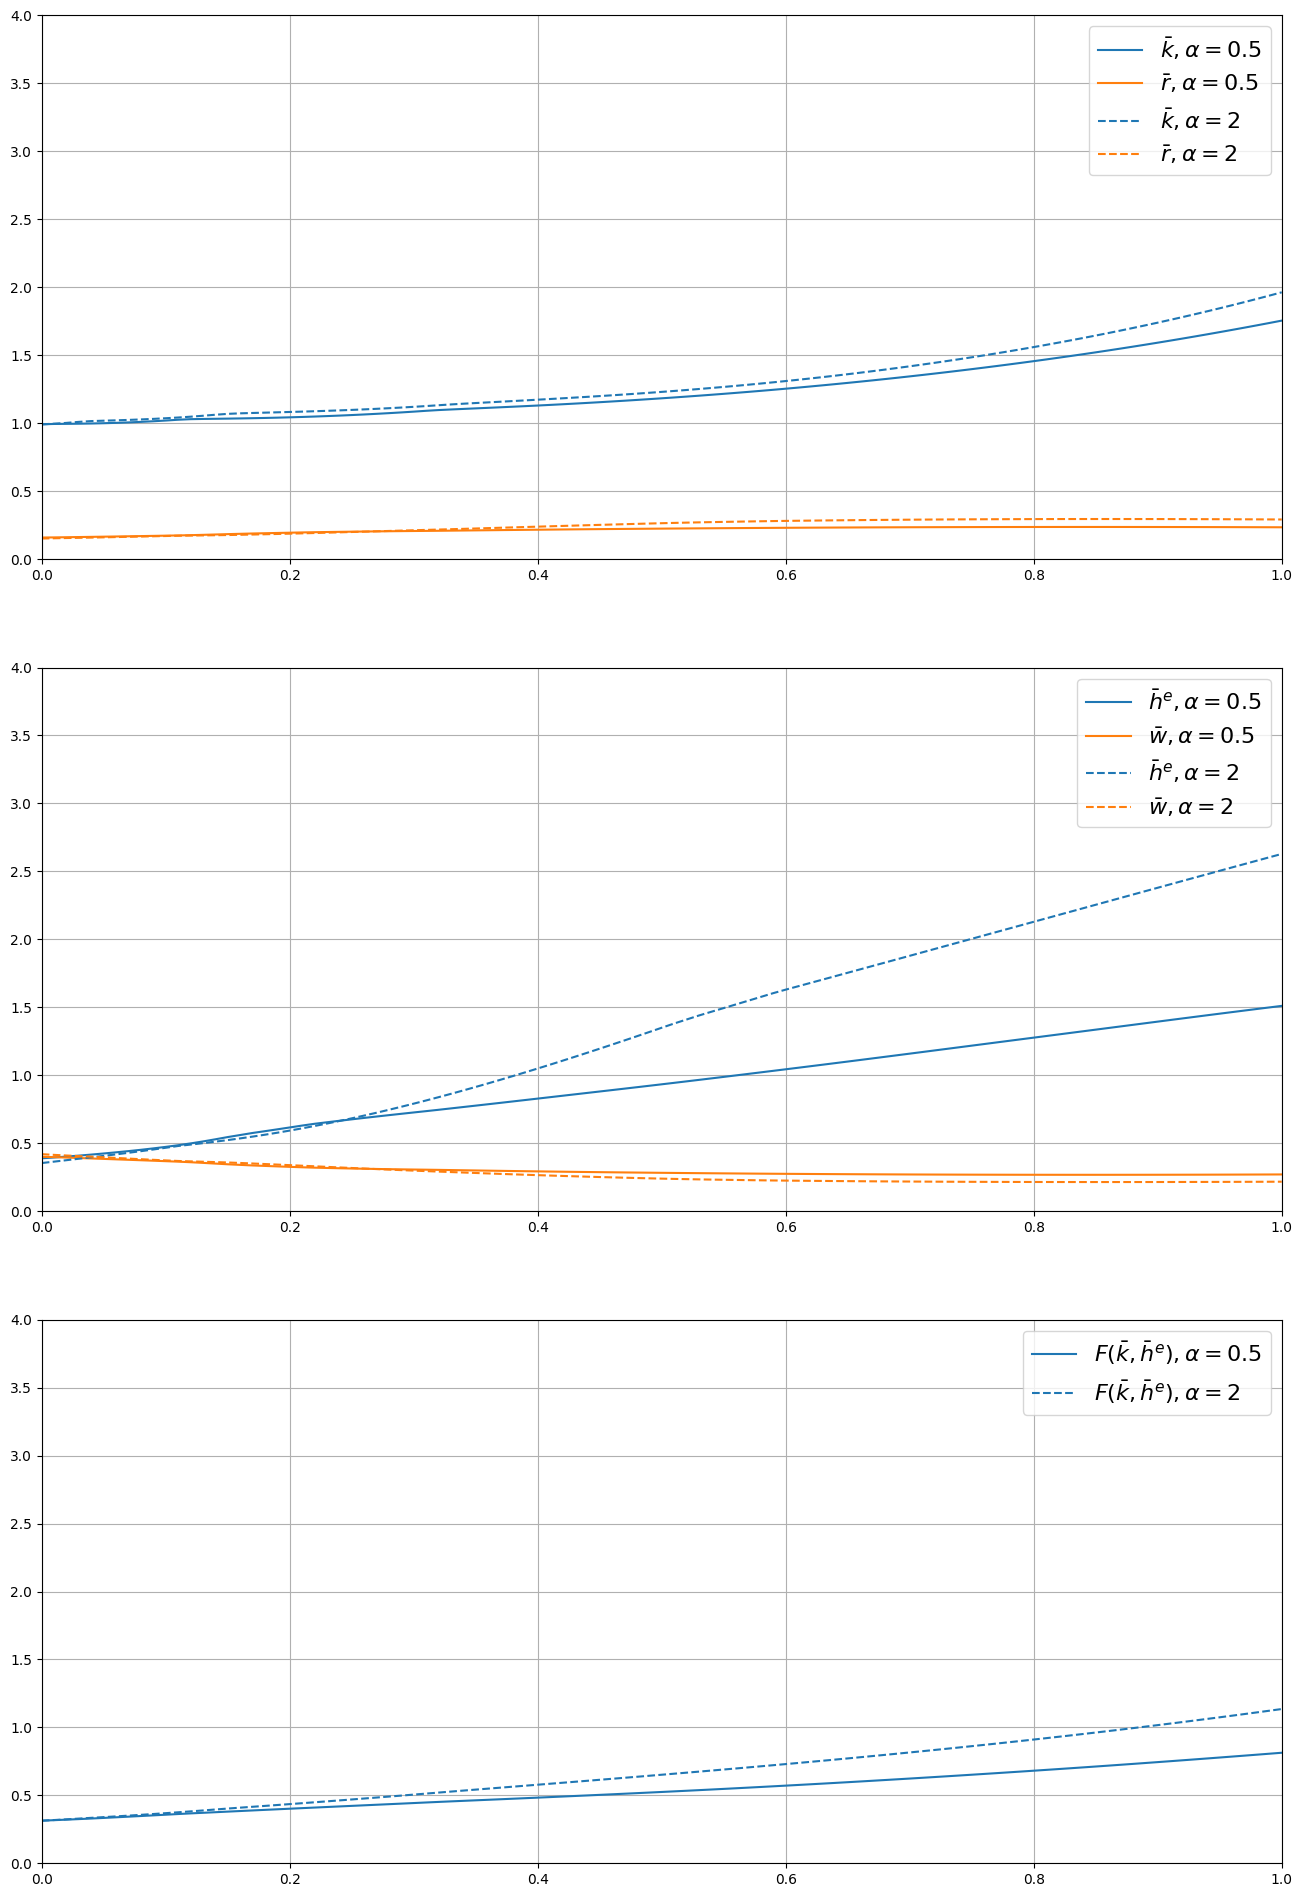
\includegraphics[width=\textwidth]{simulations_mfg.png}



\section{Conclusion}
We have reviewed mean field game theory and proposed a model of the effects of preferences for eduction in the economy.

Our next steps include simulating the full model using finite difference methods and machine learning based methods, deriving analytical results for the model, and proposing modifications to this baseline model. One such modification is to consider a principal agent mean field control problem: we could consider the scenario of a decision maker optimizing a public policy with a associated utility over the population distribution state.
\appendix
\addcontentsline{toc}{section}{Appendices}
\section*{Appendices}
\section{A brief review of game theory}\label{appendix-game-theory}

\subsubsection{Key Concepts}
\begin{enumerate}
    \item \textit{Game Theory} - area of mathematics concerned with the interaction of \textit{strategies} adopted by \textit{players} in order to maximize their \textit{payoff}. At the end of the day, a game is a system of optimization problems for which there is some interaction on the optimization target.
    \item \textit{Strategy} - an entity $x_i \in \mathcal{X}_i$ which represents one option, or control, that a player is allowed to choose, and which will be an input for the payoff function. Players want to choose their strategy in order to maximize their own payoff, while taking into account that the other players are doing the same thing.
    \item \textit{Pure vs Randomized (or mixed) Strategies}: A randomized strategy for player $i$ is a probability measure $\mu_i$ on the set of strategies $X_i$. A pure strategy is a randomized strategy with all of its mass concentrated on a single $x_i \in \mathcal{X}_i$%.  https://en.wikipedia.org/wiki/Strategy_(game_theory)#Mixed_strategy
    \item \textit{Player} - one player is equivalent to one dimension of the system of optimization problems.
    \item \textit{Payoff} - the optimization target of each player. The payoff for every player depends on the strategy chosen by every player. In the case of randomized strategies, the payoff is the expected value of the payoff function under the joint probability measure of the straties of all players.
    \item \textit{Solution concepts:} Nash Equilibrium, Stackelberg Equilibrium, Pareto Optimality.
        
        In general players cannot get the maximum payoff together. Different concepts of equilibrium are introduced in order to propose solutions to different kinds of games, which might differ by choice structure or cooperation possibility. Let`s consider the 2-dimensional case of two players, with sets of strategies denoted by $A,B$ and payoff functions $J_i: A\times B \mapsto \mathbb{R}$ for $i$ in $\{A,B\}$
    \begin{itemize}
        \item \textit{Pareto Optimality}: A pair of strategies $(a^*, b^*)$ is said to be \textbf{Pareto optimal} if there is no other pair $(a,b) \in A \times B$ such that
        $$
        J_A (a,b) > J_A(A^*, b^*) \text{ and } J_B(a,b) \geq J_B(a^*, b^*),
        $$
        or
        $$
        J_B(a,b) > J_B(a^*, b^*) \text{ and } J_A(a,b) \geq J_A(a^*,b^*).
        $$
        This means that is not possible to striclty increase the payoff of one player without strictly decreasing the payoff of the other.
        \item \textit{Nash Equilibrium}: A pair of strategies $(a^*,b^*)$ is said to be a \textbf{Nash Equilibrium} if $\forall a \in A, b\in B$, we have $J_A(a,b^*) \leq J_A(a^*,b^*)$ and $J_B(a^*,b) \leq J_B(a^*,b^*)$.
        This is a solution concept for a non-cooperative game. It is a situation in which no player can increase his payoff by changing his strategy if the other players do not change theirs. 
        \item \textit{Stackelberg Equilibrium}: Solution for a game with asymmetry of information. Let $R^B(a)$ be the set of best possible replies of Player $B$ if Player $A$ has announced the strategy $a$, that is, 
        $$R^B(a) = \{b' \in B : J_B(a,b) \leq J_B(a,b'), \forall b \in B\}.$$
        Then, a pair of strategies $(a^*,b^*) \in A\times B$ is a \textbf{Stackelberg Equilibrium} if 
        $$b^* \in R^B(a^*) \text{ and } J_A(a,b)\leq J_A(a^*, b^*),\ \forall(a,b), b\in R^B(a), a \in A.$$
    \end{itemize}
    
    \item \textit{completely cooperative and zero-sum}
    \item \textit{Information structure}: 

    % Define a differential game as setting for the strategies
    The information available for the players determine the possible strategies to be taken. This means that different game situations might arise for different information structures. Two particular information structures of notice are the \textbf{open loop} case and the \textbf{feedback case}. 
    \textbf{Open loop strategies} are strategies that depend only on time $t \in [0,T]$, which arise in situations where the state of the system cannot be known. Thus, the set $X_i$ of strategies available for the $i$-th player wiil consist of all measurable functions $t \mapsto u_i(t)$ from $[0,T]$ into $U_i$. \textbf{Feedback} (or \textbf{Markovian}) strategies arise when each player $i$ can observe the state of the system, but does not know the strategy of other players. In this case, the strategy for player $i$ can depend on both the time and the state, that is, the set of available strategies for player $i$ is the set of measurable functions $(t,x) \mapsto u_i(t,x)$ from $[0,T] \times \mathbb{R}^n$ into $U_i$ 
    \item \textit{Target and Game set}
\end{enumerate}

\end{document}